\chapter{lec07 20220225}

Topics

\begin{enumerate}
    \item Impurity spectral function: Einstein model and numerical experiment
\end{enumerate}

Goals

\begin{enumerate}
    \item First example of a physically interesting spectral function
    \item Appreciating how to ``extract'' physical info from spectral function
\end{enumerate}

Consider the state with one electron removed:
\[ \hat{c}_1|\Omega \rangle =|\left\{ 0,0,0 \right\} \rangle \otimes \prod_q{\hat{D}_{q}^{\dagger}\left( \frac{M_{1q}}{\omega _q} \right) |\left\{ 0_q \right\} \rangle _0}\]
This is \emph{not} an eigenstate of $\hat{H}$! The eigenstates should have been
\[ |\left\{ 0,0,0 \right\} \rangle \otimes |\left\{ m_q \right\} \rangle \]
Non-eigenstates means states with dynamics. So now we consider
\begin{align*}
    G_{11}\left( t \right) &=\left( -i \right) \langle \Omega |\hat{c}_{1}^{\dagger}\left( t \right) \hat{c}_1\left( 0 \right) |\Omega \rangle \\
    &=\left( -i \right) \langle \Omega |e^{i\hat{H}t}\hat{c}_{1}^{\dagger}e^{-i\hat{H}t}\hat{c}_1|\Omega \rangle \\
    &=\left( -i \right) e^{i\Delta _{100}t}\langle \Omega |\hat{c}_{1}^{\dagger}e^{-i\hat{H}t}\hat{c}_1|\Omega \rangle \\
    &=\left( -i \right) e^{i\Delta _{100}t}\left[ \langle 0_q|_0\prod_q{\hat{D}_q\left( \frac{M_{1q}}{\omega _q} \right)} \right] \otimes \langle \left\{ 100 \right\} |\hat{c}_{1}^{\dagger}e^{-i\hat{H}t}\hat{c}_1\\
    &\qquad|\left\{ 100 \right\} \rangle \otimes \prod_q{\hat{D}_{q}^{\dagger}\left( \frac{M_{1q}}{\omega _q} \right)}|\left\{ 0_q \right\} \rangle _0\\
    &=\left( -i \right) e^{i\Delta _{100}t}\left[ \langle 0_q|_0\prod_q{\hat{D}_q\left( \frac{M_{1q}}{\omega _q} \right)} \right] \exp \left\{ -i\left. \hat{H} \right|_{\left\{ 000 \right\}}t \right\}\prod_q{\hat{D}_{q}^{\dagger}\left( \frac{M_{1q}}{\omega _q} \right)}|\left\{ 0_q \right\} \rangle _0\\
\end{align*}
But
\[ \left. \hat{H} \right|_{\left\{ 000 \right\}}==\sum_q{\omega _q\hat{a}_{q}^{\dagger}\hat{a}_q}+\Delta _{000}\]
\[ \Delta _{000}=0\]
We have
\[ G_{11}\left( t \right) =\left( -i \right) e^{i\Delta _{100}t}\prod_q{\left( \langle -\frac{M_{1q}}{\omega _q}|e^{-i\omega _q\hat{a}_{q}^{\dagger}\hat{a}_qt}|\frac{M_{1q}}{\omega _q}\rangle _0 \right)}\]
where the state in the bra and ket is the coherent state. This is just the ``propagator'' in the coherent-state basis!
\begin{align*}
    G_{11}\left( t \right) &=\left( -i \right) e^{i\Delta _{100}t}\prod_q{\left( \langle -\frac{M_{1q}}{\omega _q}|\frac{M_{1q}}{\omega _q}e^{-i\omega _qt}\rangle _0 \right)}\\
    &=\left( -i \right) e^{i\Delta _{100}t}\prod_q{\exp \left( \frac{M_{1q}^{2}}{\omega _{q}^{2}}e^{-i\omega _qt} \right) \exp \left( -\frac{M_{1q}^{2}}{\omega _{q}^{2}} \right)}
\end{align*}
Let's define $g_q=\left( \frac{M_{1q}}{\omega _q} \right) ^2$, then
\[ G_{11}\left( t \right) =\left( -i \right) e^{i\Delta _{100}t}\exp \left( \sum_q{g_q\left( e^{-i\omega _qt}-1 \right)} \right) \]
To make further progress, consider again the Einstein model with
\[ \omega _q=\omega _E,\quad \forall q\]
Let $g=\sum_q{g_q}$, then
\[ G_{11}\left( t \right) =\left( -i \right) e^{i\Delta _{100}t}\exp \left( ge^{-i\omega _Et}-g \right) \]
We can now consider the Fourier transform
\begin{align*}
    G_{11}\left( \omega \right) &=\left( -i \right) e^{-g}\lim_{\eta \rightarrow 0^+} \int_0^{\infty}{dte^{i\Delta _{100}t}e^{i\omega t}e^{-\eta t}\exp \left( ge^{-i\omega _Et} \right)}\\
    &=\left( -i \right) e^{-g}\sum_{l=0}^{\infty}{\lim_{\eta \rightarrow 0^+} \int_0^{\infty}{dt\frac{g^l}{l!}e^{i\left( \omega +\Delta _{100}-l\omega _E+i\eta \right) t}}}\\
    &=e^{-g}\sum_{l=0}^{\infty}{\lim_{\eta \rightarrow 0^+} \frac{g^l}{l!}\frac{1}{\omega +\Delta _{100}-l\omega _E+i\eta}}\\
\end{align*}
and same as before we find the spectral function
\begin{align*}
    A_{11}\left( \omega \right) &=\frac{-1}{\pi}\mathrm{Im}G_{11}\left( \omega \right) \\
    &=\sum_{l=0}^{\infty}{e^{-g}\frac{g^l}{l!}\delta \left( \omega -\left( -\Delta _{100}+l\omega _E \right) \right)}
\end{align*}
\[ \Delta _{100}=\varepsilon _1-\sum_q{\frac{M_{1q}^{2}}{\omega _q}}=\varepsilon _1-\omega _Eg<0\]
The spectral function is the sum of delta functions. For which $l$ do we get the highest weight?
\[ \frac{g^{l+1}}{\left( l+1 \right) !}=\left( \frac{g}{l+1} \right) \left( \frac{g^l}{l!} \right) \]
increasing for $l<g-1$, decreasing for $l>g-1$

\begin{figure}[ht]
    \centering
    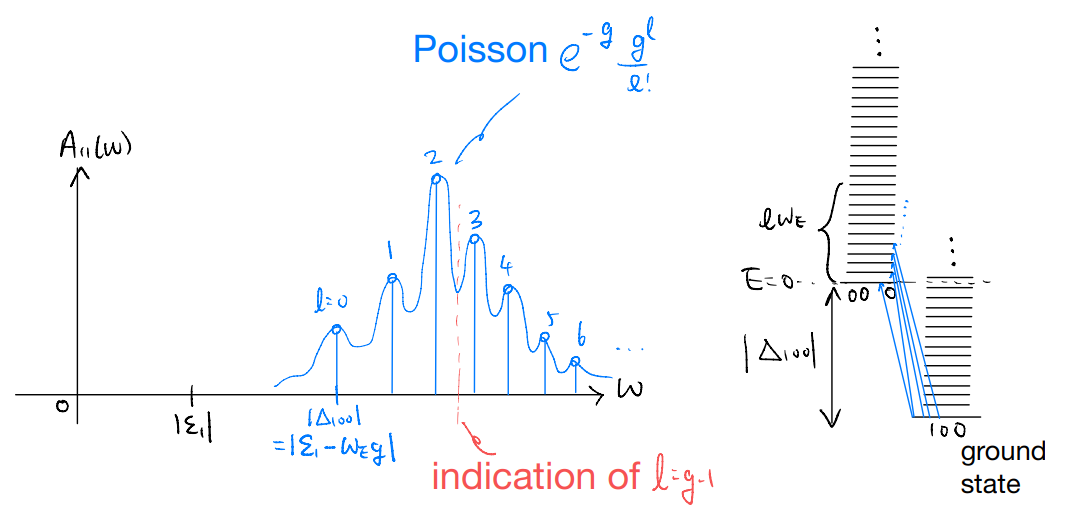
\includegraphics[width=\textwidth]{jupyterbook/data/fig/lec07-fig00.png}
\end{figure}

Interpretation: when we try to remove an electron, we discover that in the ground state the "electron" is actually dressed by the phonons. With strong coupling ($g\gg 1$), the dominant spectral peak is far from the bare electronic orbital contribution of $|\Delta_{100}|$.

Notes:
\begin{enumerate}
    \item The Einstein model is simple by design, and enables very explicit computation of the frequency-space Green's function (and hence spectral function). Our real-time solution, however, holds for more general phonon dispersion. When we deviate from the Einstein model we should start seeing deviation from the ``sum of delta function'' form of the spectral function
    \item More interestingly, one should ask what happens for acoustic phonons which have $\omega_q\to 0$ as $q\to 0$. Recall the strength of the $e-ph$ coupling was parameterized by $g_q=\left(\frac{M_{iq}}{\omega_q}\right)^2$. If $M_{iq}$ stays finite and $\omega_q\to 0$, we have diverging coupling and hence energies etc.!
\end{enumerate}

This is a rather general feature: low-energy modes are ``dangerous'' because they are easy to excite. In finding the ground state, one should, generally speaking, check how the ``fluctuations'' (lowest excitations) could destabilize the ground state. This amounts to a kind of self-consistency check. If the assumed ground state implies strong fluctuations which kills itself, the ground state does not actually ``form''. This is the key physical picture behind the Merlin-Wagner theorem on the absence of spontaneous continuous symmetry breaking in low dimensions.

Now, back to our impurity-phonon problem: physically, the acoustic phonons have vanishing frequency in the long-wavelength limit because they are Goldstone modes. The Goldstones exist because of symmetries, and are correspondingly constrained by symmetries. In our context, the catastrophe is avoided by having a ``derivative coupling'', such that the $e-ph$ coupling has a momentum dependence of $M_{iq}\propto q$ as $q\to 0$. This gives a finite coupling strength as both $M_{iq}$ and $\omega_q$ vanish linearly in $q$.

Note: play with the uploaded Python code if you want to explore what happens beyond the Einstein model.
